\documentclass[pdftex,12pt,a4paper]{report}
\usepackage[pdftex]{graphicx}
\usepackage{hyperref,pdfpages}
\usepackage[english]{babel}
\usepackage[left=2cm,top=1cm,right=3cm,nohead]{geometry}

\newcommand{\HRule}{\rule{\linewidth}{0.5mm}}

\begin{document}



\begin{titlepage}
\begin{center}

\textsc{\LARGE [CSC318H1]}\\[0.5cm]
\textsc{The Design of Interactive Computational Media}\\[1cm]

\textsc{\Large TA: Christina Christodoulaki}\\[0.5cm]

% Title
\HRule \\[0.4cm]
{ \huge \bfseries Haptic5 Evaluation Report}\\[0.4cm]

\HRule \\[1.5cm]

% Author and supervisor
\begin{minipage}{0.4\textwidth}
\begin{flushleft} \large
\emph{Haptic5 Members:}\\
Taylor\textsc{ Dickson}\\
Victoria\textsc{ Enalen}\\
Wilson\textsc{ Sun}\\
Zhi\textsc{ Zhang}\\
Lia\textsc{ Zheng}\\
\end{flushleft}
\end{minipage}
\begin{minipage}{0.4\textwidth}
\begin{flushright} \large
\emph{Emails:} \\
 me@taylordickson.ca\\
 enalenv@gmail.com \\
 wilson.sun@hotmail.ca\\
 cakyo@live.ca‎\\
 citrus.smooth@gmail.com\\
 
\end{flushright}
\end{minipage}

\vfill

% Bottom of the page
{\large \today}

\end{center}
\end{titlepage}
\tableofcontents

\chapter{Heuristic Evaluation}
A heuristic evaluation was carried out during the February 26th CSC318 tutorial in order to assess conformity of our application to the 5 usability heuristics we have identified as important. This evaluation employed 5 expert evaluators who were asked to complete 2 pre-determined task on paper prototypes and provide feedback based on the 5 heuristics.

\section{Rationale}
Our rationale for using a heuristic evaluation is that the feedback provided by these expert evaluators would yield a greater benefit with a small number of participants leading to decreased time spent. \footnote{As seen on slide 34 in Lecture 6: Usability Principles \& Heuristic Evaluations}

\section{Participants}
We recruited 5 expert evaluators from our CSC318 course at the University of Toronto. These evaluators are male between the ages of 20 to 25. Four of the evaluators are on their way to completing a Computer Science major/specialist, one did not disclose his information. It is important to note that all evaluators are comfortable using a smartphone, as they all own a smartphone, with 2 of the 5 evaluators running iOS on their smartphone, and the rest running an android operating system. These expert evaluators are also quite familiar with heuristic evaluations and are comfortable with the 5 usability heuristics that were explained to them at the start of the usability task.
\section{Usability Criteria}

To carry out the heuristic evaluation we first presented the evaluators with a description of the 5 usability criteria and how they would be important to our application. These criteria are as follows:
\vspace{0.7cm}

\noindent\textbf{[Consistency and Standards]}
\vspace{0.2cm}
\\The icons and actions that are available must be consistent with what the user thinks
the resulting action should be. The icons and actions should also have uniform
meaning throughout the use of the application and relate to the current platform
so as not to confuse the user and to make available actions recognizable.
\pagebreak
\\\textbf{[Flexibility and Efficiency]}
\vspace{0.3cm}
\\The application must have the ability to customize interaction in order to conform
to the current user. Implementation of this is important in order to have quick user
response times and to accommodate all types of users.
\vspace{0.7cm}
\\\textbf{[Error Prevention]}
\vspace{0.3cm}
\\With a restricted set of actions and the ability to edit data, we can ensure that
the user is never confronted with any form of error. While the data input is up to
the users themselves, the app should always provide means of editing data and to
limit choices, for example with the use of radio buttons. Keeping the data collection
methods consistent prevents the application from raising any form of error.
\vspace{0.7cm}
\\\textbf{[Visibility of System Status]}
\vspace{0.3cm}
\\The user should always know of the current status of the application and what
actions are available at that time. Properly titled pages along with current system
readiness, such as an hourglass to indicate that the system is working or busy, will
let the user know what is happening at that very moment.
\vspace{0.7cm}
\\\textbf{[Aesthetic and Minimal Design]}
\vspace{0.3cm}
\\Eliminating unnecessary actions and icons can reveal what the user is able to do at
that moment in time. Since the interface will have a reduced number of actions, it is
relatively easy to keep the screen visually pleasing and at the same time informative,
letting the user know that the only available actions are the ones seen on the screen.

\section{Tasks}
The evaluators were then asked to complete 2 tasks on the paper prototypes. The evaluators were presented with the home screen at the start of each task, and simulation of the task occurred via the evaluator's interaction with the ``buttons'' on the protoype. Tapping on the keyboard button allows the evaluator to simulate typing on the screen, and tapping on action buttons would present the evaluator with another screen prototype. \footnote{The screen prototypes can be found in the Appendix} The tasks given are as follows:
\vspace{0.7cm}
\\\textbf{Task 1:} Log into the application, get to the log entry screen and complete an entry.
This is performed by tapping on application icon shown in \textit{Screen 1}, inputting a password
if necessary (the details for the password are already given) or choosing a user that does
not have a password (seen in \textit{Screen 4}) and by clicking Add New shown in \textit{Screen 5}. From here it brings the user to the entry screen as seen on \textit{Screen 6} where the user can input data and confirm their entry by clicking OK as seen on \textit{Screen 7}.
\vspace{0.7cm}
\\\textbf{Task 2:} Create a custom category to add to the log entry screen. From the home screen
\textit{Screen 5}, the user should click the Settings icon on the top right-hand corner which will
bring them to \textit{Screen 10}. Users should then click Change Log (bringing them to \textit{Screen 12}) and then click Create New.

\chapter{Cognitive Evaluation}
We conducted a cognitive evaluation with 5 expert evaluators to assess the learnability of our system. An interaction task was selected and an appropriate sequence was determined so that our users were able to answer our 4 questions based on our paper prototypes.

\section{Rationale}
We chose to employ the cognitive evaluation to assess learnability of the system for first time users. Since the cognitive evaluation uses expert evaluators we are gaining an increased amount of relevant feedback for a decreased amount of time spent in recruiting and working with the evaluators.

\section{Task}

The evaluators were told that the task was to create a new entry. We started off each evaluator with the home screen, and at each step of the task we asked each evaluator the four questions to assess learnability of the system, and produced the appropriate screen protype as the task progressed. 
\vspace{0.7cm}
\\Task 1: Create a new entry. 
\\Interaction Sequence:
\vspace{0.3cm}
 \\(0) Open application.  \textit{Screen 1}
 \\(1) Type Credentials \textit{Screen 3}
 \\(2) Click ``okay''.  \textit{Screen 3}
 \\(3) Click ``Add New'' button.  \textit{Screen 5}
 \\(4) Fill out entry.  \textit{Screen 9}
 \\(5) Click ``OK!''.  \textit{Screen 8}
\vspace{0.7cm}

The following four questions were asked to create a believability story for each step of interaction sequence:
\vspace{0.7cm}
\\(a) Will the user be trying to produce whatever effect the action has?
\\(b) Will the user be able to notice that the correct action is available?
\\(c) Once the user finds the correct action at the interface, will she know that it is the right one for the effect she is trying to produce?
\\(d) After the action is taken, will the user understand the feedback given?

\section{Participants}
Five expert evaluators were recruited from the Great Hall of Computing, 3 males, and 2 females between the ages of 21-24. All of the evaluators are in the Computer Science major, and four of the evaluators were familiar with the cognitive evaluation process. All of the evaluators were comfortable using a smartphone with 3 of them running iOS, and 2 of them running the android system.
\chapter{Think-aloud Evaluation}
A think aloud is a very straightforward process that requires only a participant and the paper prototype for the application. It involves the participant executing a given task while giving verbal feedback of all actions and thoughts encountered. For a think aloud, speech throughout the entire task is encouraged and needed to gather accurate, user-perspective data. In order for the participants to be comfortable with verbalizing their actions and their thoughts, we provide a few practice sessions involving objects not related to the application in order for them to get used to speaking their actions.

To ensure an accurate presentation of the think aloud for each participant, we have generated a script that will be presented to each participant. The script consists of a basic description that is given to all participants along with practice tasks that can be given until the participant is comfortable with thinking out loud. The practice sessions use a basic calculator since it is an object that most people are familiar with. The familiarity will help users be confident of their actions and pick up the task more readily. The think aloud itself will only require the paper prototype.

\section{Think Aloud Script}
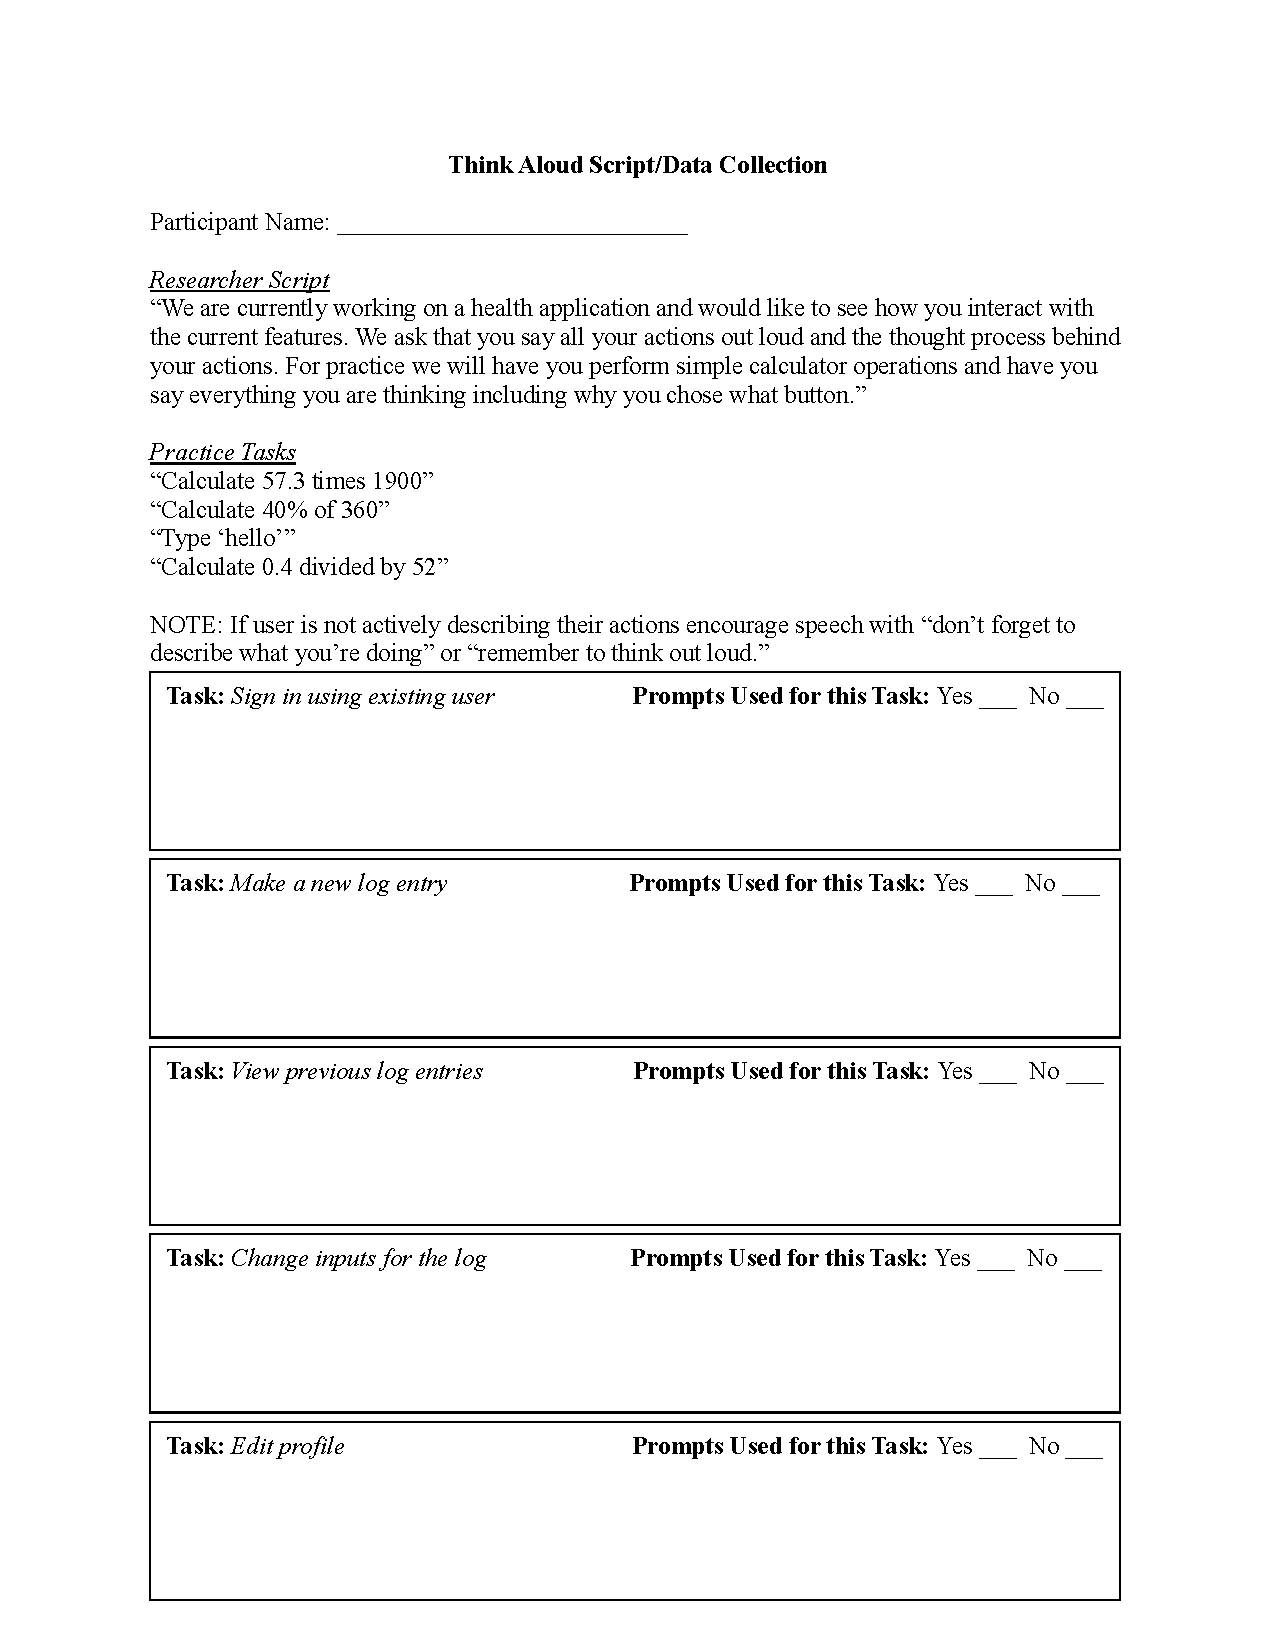
\includepdf[pages=-]{Screens/ThinkAloudScript.pdf}

\section{Rationale}
Performing a think aloud is suitable for our application's current state since it allows us to gather data without needing any additional equipment; only the paper prototype and a participant is required. Also, since this method is quick and easy to perform, we are able to gather numerous participants and keep explanation of the task at hand to a minimum.
\section{Tasks}
\begin{itemize}
\item Sign in using existing user
\item Make a new log entry
\item View previous log entries
\item Change inputs for the log
\item Edit profile
\end{itemize}
\section{Participants}
The participants gathered for the think aloud varied in age: three of the five participants were aged 20-25 and the remaining two were between 40 and 45. The evaluators between the ages of 20 and 25 are currently attending post-secondary institutions while the remaining evaluators are currently working full time. All participants do own and operate smart phones, but only do so for their basic features. This implies that the users know basic smart phone maneuvering, but are not ``experts'' in any one task. None of the participants were previously exposed to the application in any form and will be seeing it for the first time while doing the think aloud.\\

\chapter{Results}
\section*{Heuristic Evaluation Results}
\textbf{Task 1}
\begin{center}
	\begin{tabular}{|p{\textwidth}|}
	\hline
	\textbf{User}: Student 1\\
	\hline
	\textbf{Name}: The term \emph{Add New} is ambiguous\\
	\hline
	\textbf{Problem/Good Aspect}: Problem\\
	\hline
	\textbf{Evidence}:
	\begin{itemize}
	\item{User managed to log in correctly and without problem, but when presented with the home screen he hesitated to \emph{Add New} stating ``Add new what?''}
	\item{Eventually it was tapped (mostly out of the large prominent nature of the button) and it brought him to the correct screen}
	\end{itemize}\\
	\hline
	\textbf{Explanation}:\\
	The user was able to log into the home page of the screen but was hesitant in pressing \emph{Add New} as, to him, it wasn't clear where clicking that button would take him. However, since the button took up the majority of the screen, he clicked the button resulting in the correct action. Once in the screen, he seemed to be more comfortable with the controls as he was able to complete and submit an entry. The overall time it took to complete this task was very short (ie: under a minute), but there were unclear segments as indicated by the user.\\
	\hline
	\textbf{Severity or Benefit}:
	\begin{itemize}
	\item{Rating: 2, minor usability problem}
	\end{itemize}
	\textbf{Justification(Frequency, Impact, Persistence)}:
	\begin{itemize}
	\item{\textbf{Frequency}:} Low - Only new users will not know the meaning of \emph{Add New} until clicked
	\item{\textbf{Impact}:} Low - Confusing at first, but users can click the button with no consequence
	\item{\textbf{Persistence}:} Low - After clicking the icon once, users will associate the action with the button
	\end{itemize}
	\textbf{How these factors are weighted and why}:\\
	All categories are low because of the fact that users will quickly learn what Add New does and there is no harmful consequence in clicking the button to begin with. Because of this, the problem can be considered a minor usability problem.\\
	\hline
	\textbf{Possible solution and/or trade-offs}:\\
	Make the \emph{Add New} button less ambiguous by using more descriptive text.\\
	\hline
	\end{tabular}
\end{center}

\begin{center}
	\begin{tabular}{|p{\textwidth}|}
	\hline
	\textbf{User}: Student 2\\
	\hline
	\textbf{Name}: Log-in Screen buttons are misplaced with ambiguous text\\
	\hline
	\textbf{Problem/Good Aspect}: Problem\\
	\hline
	\textbf{Evidence}:
	\begin{itemize}
	\item{User struggled to log on, and pressed cancel the first time. Once he logged on he was able to navigate into "Add New" and fill out a new log. The user let out an angry sigh before saving the log.}
	\end{itemize}\\
	\hline
	\textbf{Explanation}:\\
	because he felt compelled to press on the left-most button that on our application is labelled "Cancel", stating that it is convention to have the affirmative action on the left side, and it should be labelled "Sign-in" or "Log-on" rather than "Okay". The user also had a problem with the "Ok!" button when saving the log, he felt it needed to be less ambiguous.\\
	\hline
	\textbf{Severity or Benefit}:
	\begin{itemize}
	\item{Rating: 3, major usability problem}
	\end{itemize}
	\textbf{Justification(Frequency, Impact, Persistence)}:
	\begin{itemize}
	\item{\textbf{Frequency}:} High - The user was unable to sign-in the first time and had to try again, he will be presented with this problem each time he signs on.
	\item{\textbf{Impact}:} Moderate - It caused the user to be frustrated at the application for not following standards.
	\item{\textbf{Persistence}:} None - Once signed on the user may continue without encountering the same problem.
	\end{itemize}
	\textbf{How these factors are weighted and why}:\\
	The aim of the application is to be intuitive, having a user struggle during the logging in process detracts from this goal, and the frequency of encountering this problem occurs each time the application is opened so this poses a major usability problem.\\
	\hline
	\textbf{Possible solution and/or trade-offs}:\\
Can switch around the order of the buttons, and label the affirmative action "Sign-in". Can also label "Ok!" button in the new entry as "Save log".\\
	\hline
	\end{tabular}
\end{center}

\begin{center}
	\begin{tabular}{|p{\textwidth}|}
	\hline
	\textbf{User}: Student 3\\
	\hline
	\textbf{Name}: The big plus sign is misleading and home screen should be different\\
	\hline
	\textbf{Problem/Good Aspect}: Problem\\
	\hline
	\textbf{Evidence}:
	\begin{itemize}
	\item{``What does the big plus sign mean? Is that where you would add a new custom category?''}
	\item{``Why wouldn't logging in bring me directly to the entry screen?''}
	\end{itemize}\\
	\hline
	\textbf{Explanation}:\\
	This user is more familiar with the goal and implementations of the app, but was confused as to why logging in wouldn't bring him to the entry screen. When confronted with the home screen, further confusion was met with the large plus sign on the \emph{Add New} button. The user clicked it in order to get to the correct screen, but there were questions as to why things were placed the way that they were.\\
	\hline
\textbf{Severity or Benefit}:
	\begin{itemize}
	\item{Rating: 2, minor usability problem}
	\end{itemize}
	\textbf{Justification(Frequency, Impact, Persistence)}:
	\begin{itemize}
	\item{\textbf{Frequency}:} Low - If the user has not seen the screen layout before, the icons and screen order will seem ambiguous, but only upon first use
	\item{\textbf{Impact}:} Low - Users can simply click the button to find out what it does with no consequence
	\item{\textbf{Persistence}:} Low - Once discovering what the button does, the user can become accustomed to the action and the screen order
	\end{itemize}
	\textbf{How these factors are weighted and why}:\\
	Again, all these categories are rated low because of the one-time occurrence of the problem and as such it is a minor usability problem.\\
	\hline
	\textbf{Possible solution and/or trade-offs}:
	\begin{itemize}
	\item{Make the \emph{Add New} button less ambiguous by using more descriptive text.}
	\item{Give the option to show the entry screen upon login as opposed to the given home screen}
	\end{itemize}\\
	\hline
	\end{tabular}
\end{center}

\begin{center}
	\begin{tabular}{|p{\textwidth}|}
	\hline
	\textbf{User}: Student 4 \& Student 5\\
	\hline
	\textbf{Name}: No difficulty in navigating the task.\\
	\hline
	\textbf{Problem/Good Aspect}: Good\\
	\hline
	\textbf{Evidence}:
	\begin{itemize}
	\item{Both users were able to log on, navigate to a new entry, and make said entry very quickly.}
	\end{itemize}\\
	\hline
	\textbf{Explanation}:\\
	Both users were very comfortable with the android system. Student 4 said that everything looked to be clearly labelled. Student 5 thought his success was trivial.\\
	\hline
\textbf{Severity or Benefit}:
	\begin{itemize}
	\item{Rating: 0, not a usability problem.}
	\end{itemize}
	\textbf{Justification(Frequency, Impact, Persistence)}:
	\begin{itemize}
	\item{\textbf{Frequency}:} None - There were no issues that arose.
	\item{\textbf{Impact}:} None - No problem impact, only a positive one.
	\item{\textbf{Persistence}:} None - No issue persisted.
	\end{itemize}
	\textbf{How these factors are weighted and why}:\\
	Since the user did not encounter any problems, this is not considered a usability problem.\\
	\hline
	\textbf{Possible solution and/or trade-offs}:
	\begin{itemize}
	\item{N/A}
	\end{itemize}\\
	\hline
	\end{tabular}
\end{center}

\textbf{Task 2}
\begin{center}
	\begin{tabular}{|p{\textwidth}|}
	\hline
	\textbf{User}: Student 1\\
	\hline
	\textbf{Name}: Can't find the \emph{Settings} screen\\
	\hline
	\textbf{Problem/Good Aspect}: Problem\\
	\hline
	\textbf{Evidence}:
	\begin{itemize}
	\item{User went back and forth between screens the log entry screen and home screen before noticing the settings icon on the top right.}
	\item{Once in the \emph{Settings} screen, user scanned through the categories but did not know where he could add a custom category for the log entry.}
	\end{itemize}\\
	\hline
	\textbf{Explanation}:\\The user assumed that the settings for the log entries would be located in the log entry page, but could not find it. Instead of trying other options, the user went back and forth between the home page and the entry page hoping to see a clue that would lead him in the right direction. Eventually the icon was found on the home screen, but upon getting to the \emph{Settings} screen, the user did not know which category would complete the task because of the menu labeling.\\
	\hline
\textbf{Severity or Benefit}:
	\begin{itemize}
	\item{Rating: 3, major usability problem}
	\end{itemize}
	\textbf{Justification(Frequency, Impact, Persistence)}:
	\begin{itemize}
	\item{\textbf{Frequency}:} Moderate/High - This may occur every time the user wishes to change their entry settings
	\item{\textbf{Impact}:} High - The user was clearly confused in finding this setting and only overcame the issue once he scrutinized the screens. If the user wanted to do this quickly, he may end up giving up because of the complexity. 
	\item{\textbf{Persistence}:} Moderate - The user will get used to the settings menu over time, but because it is inconveniently placed, it is still a concern.
	\end{itemize}
	\textbf{How these factors are weighted and why}:\\
	Since customization is a key point in this application, the moderate/high frequency of this issue is followed by a high impact and moderate persistence leaving this to be a major usability problem.\\
	\hline
	\textbf{Possible solution and/or trade-offs}:\\
	Make the \emph{Settings} icon more prominent and available on every screen or give the user the direct ability to create a custom data field right from the log entry screen. This may reduce the minimalistic feel of the application, but it will increase it's convenience and functionality.\\
	\hline
	\end{tabular}
\end{center}

\begin{center}
	\begin{tabular}{|p{\textwidth}|}
	\hline
	\textbf{User}: Student 2\\
	\hline
	\textbf{Name}: No problems with task.\\
	\hline
	\textbf{Problem/Good Aspect}: Good.\\
	\hline
	\textbf{Evidence}:
	\begin{itemize}
	\item{User was able to find the settings icon and create a new custom log item.}
	\end{itemize}\\
	\hline
	\textbf{Explanation}:\\The user thought the task was intuitive as changing settings would "obviously be found in the settings menu".\\
	\hline
\textbf{Severity or Benefit}:
	\begin{itemize}
	\item{Rating: 0, not a usability problem}
	\end{itemize}
	\textbf{Justification(Frequency, Impact, Persistence)}:
	\begin{itemize}
	\item{\textbf{Frequency}:} None - No usability problem.
	\item{\textbf{Impact}:} None - No impact.
	\item{\textbf{Persistence}:} None - Lack of problem does not persist.
	\end{itemize}
	\textbf{How these factors are weighted and why}:\\
	As there is no problem, rated 0.\\
	\hline
	\textbf{Possible solution and/or trade-offs}:\\
	N/A\\
	\hline
	\end{tabular}
\end{center}

\begin{center}
	\begin{tabular}{|p{\textwidth}|}
	\hline
	\textbf{User}: Student 3\\
	\hline
	\textbf{Name}: Problematic labeling within \emph{Settings}\\
	\hline
	\textbf{Problem/Good Aspect}: Problem\\
	\hline
	\textbf{Evidence}:
	\begin{itemize}
	\item{User was able to find the \emph{Settings} icon quickly}
	\item{User clicked \emph{Medical History} first before clicking \emph{Change Log}, but was able to find the screen that would create a custom category.}
	\item{This user suggested that we call \emph{Change Log} ``Edit Categories'' instead}
	\end{itemize}\\
	\hline
	\textbf{Explanation}:\\This user has seen the screenshots before (during the CSC318 presentation) and was familiar with the different functions of the app. He had no trouble getting to the \emph{Settings} screen, but initially clicked \emph{Medical History} before \emph{Change Log}. Because of this error, he suggested that we call the category something more descriptive such as ``Edit Categories.''\\
	\hline
\textbf{Severity or Benefit}:
	\begin{itemize}
	\item{Rating: 2, minor usability problem}
	\end{itemize}
	\textbf{Justification(Frequency, Impact, Persistence)}:
	\begin{itemize}
	\item{\textbf{Frequency}:} Moderate/High - Users will want to utilize the customization feature very frequently
	\item{\textbf{Impact}:} Moderate - Not being able to quickly find this feature will limit the capability of the app greatly
	\item{\textbf{Persistence}:} Low - The user will quickly learn the functions of each category
	\end{itemize}
	\textbf{How these factors are weighted and why}:\\
	Since the user was able to overcome the issue quickly, the persistence of this issue for this user is low thus balancing the high frequency. This leads this issue to be a minor usability problem for this user.\\
	\hline
	\textbf{Possible solution and/or trade-offs}:\\
	Make the \emph{Change Log} setting less ambiguous by using more descriptive text.\\
	\hline
	\end{tabular}
\end{center}


\begin{center}
	\begin{tabular}{|p{\textwidth}|}
	\hline
	\textbf{User}: Student 4\\
	\hline
	\textbf{Name}: Location of custom category not intuitive.\\
	\hline
	\textbf{Problem/Good Aspect}: Problem\\
	\hline
	\textbf{Evidence}:
	\begin{itemize}
	\item{The user took a bit of time finding the settings button, but then was able to create a new custom category very easily.}
	\end{itemize}\\
	\hline
	\textbf{Explanation}:\\
	The user narrowed down the settings button as the location of creating a new custom category because he didn't remember there being an option in the entry itself, and from there he found the task easy.\\
	\hline
\textbf{Severity or Benefit}:
	\begin{itemize}
	\item{Rating: 1, minor usability problem}
	\end{itemize}
	\textbf{Justification(Frequency, Impact, Persistence)}:
	\begin{itemize}
	\item{\textbf{Frequency}:} Low - A new user may not think that a new custom category could be created under settings.
	\item{\textbf{Impact}:} Low - Causes the user to think about where the feature would be found.
	\item{\textbf{Persistence}:} Low - After finding it the first time around the user will be able to adapt.
	\end{itemize}
	\textbf{How these factors are weighted and why}:\\
	Since all categories are rated low, this consists as a minor usability issue, particularly because it did not hinder the user from the task.\\
	\hline
	\textbf{Possible solution and/or trade-offs}:
	\begin{itemize}
	\item{Can add an option to add a custom category from the entry log itself so the user do not need to navigate to find the feature.}
	\end{itemize}\\
	\hline
	\end{tabular}
\end{center}

\begin{center}
	\begin{tabular}{|p{\textwidth}|}
	\hline
	\textbf{User}: Student 5\\
	\hline
	\textbf{Name}: Settings button not visible.\\
	\hline
	\textbf{Problem/Good Aspect}: Problem\\
	\hline
	\textbf{Evidence}:
	\begin{itemize}
	\item{The user navigated back to Add New, and to Previous Days with no luck.}
	\item{User did not complete the task.}
	\end{itemize}\\
	\hline
	\textbf{Explanation}:\\
	The user did not realize the settings icon was a button, and thought it was part of the logo.\\
	\hline
\textbf{Severity or Benefit}:
	\begin{itemize}
	\item{Rating: 4, major usability problem}
	\end{itemize}
	\textbf{Justification(Frequency, Impact, Persistence)}:
	\begin{itemize}
	\item{\textbf{Frequency}:} Moderate - A non-android user might not recognize the settings icon.
	\item{\textbf{Impact}:} High - Caused the user to be unsuccessful at the task.
	\item{\textbf{Persistence}:} Low - After usage of other android applications the user will be able to relate to the icon.
	\end{itemize}
	\textbf{How these factors are weighted and why}:\\
	Impact of this issue is weighed the highest because we do not want a user to give up on a functionality of our application, thus this is considered a major usability problem.\\
	\hline
	\textbf{Possible solution and/or trade-offs}:
	\begin{itemize}
	\item{Possible to add a text below the icon, or have it highlighted in another colour to increase visibility.}
	\end{itemize}\\
	\hline
	\end{tabular}
\end{center}

\section*{Cognitive Evaluation Results}

\begin{center}
State 0 (Open Application - Screen 1)
\end{center}

(a) Will the user be trying to produce whatever effect the action has?
\\\indent \textbf{Student 1:} Yes, if they want to use the application.
\\\indent \textbf{Student 2:} Sure, to use the app.
\\\indent \textbf{Student 3:} Obviously? Doesn't the user want to use the app?
\\\indent \textbf{Student 4:} Yes, because the application must be open in order to be used.
\\\indent \textbf{Student 5:} Yes, if they are seeking to utilize the application.
\\(b) Will the user be able to notice that the correct action is available?
\\\indent \textbf{Student 1:} Yes, there is an icon on the screen.
\\\indent \textbf{Student 2:} Yeah, there's the logo.
\\\indent \textbf{Student 3:} Yes, that symbol looks like it can be "opened".
\\\indent \textbf{Student 4:} Yes, because the application must be open in order to be used.
\\\indent \textbf{Student 5:} Yes, the android user can see the application icon.
\\(c) Once the user finds the correct action at the interface, will she know that it is the right one for the effect she is trying to produce?
\\\indent \textbf{Student 1:} Yes, if they want to use the application.
\\\indent \textbf{Student 2:} Sure, to use the app.
\\\indent \textbf{Student 3:} Yes, there's one button.
\\\indent \textbf{Student 4:} Yes, because it's the only thing on the screen.
\\\indent \textbf{Student 5:} Yes. An android user understands that tapping on the application icon opens it up.
\\(d) After the action is taken, will the user understand the feedback given?
\\\indent \textbf{Student 1:} Yes, if the user knows that Haptic5 is the name of the application.
\\\indent \textbf{Student 2:} Yeah, the app is open duh.
\\\indent \textbf{Student 3:} Yes, the screen has changed.
\\\indent \textbf{Student 4:} No, there's a lock symbol so technically the application isn't fully open.
\\\indent \textbf{Student 5:} Yes, the welcome page is open.

\begin{center}
	\begin{tabular}{|p{\textwidth}|}
	\hline
	\textbf{User}: Student 4\\
	\hline
	\textbf{Name}: Lock symbol denotes application isn't open.\\
	\hline
	\textbf{Problem/Good Aspect}: Problem\\
	\hline
	\textbf{Evidence}:
	\begin{itemize}
	\item{Task Step 0:Open application.  \textit{Screen 1}}
	\item{Question: After the action is taken, will the user understand the feedback given?}
	\end{itemize}\\
	\hline
	\textbf{Explanation}:\\
	The user goes to open the application and then is presented with a lock sign, so that indicates the application isn't open. \\
	\hline
	\textbf{Severity or Benefit}:
	\begin{itemize}
	\item{Rating: 0, Not a usability problem}
	\end{itemize}
	\textbf{Justification(Frequency, Impact, Persistence)}:
	\begin{itemize}
	\item{\textbf{Frequency}:} Low - This may be a problem for a novice user and may be confusing.
	\item{\textbf{Impact}:} Low - Confusing at first, but users can click the lock button with no consequence thereafter.
	\item{\textbf{Persistence}:} Low - Problem does not persist after the first time.
	\end{itemize}
	\textbf{How these factors are weighted and why}:\\
	All categories are low because this is more of a technicality in the word open, rather than a usability problem. Perhaps novice users may encounter confusion with the lock symbol.\\
	\hline
	\textbf{Possible solution and/or trade-offs}:\\
	Include a header that says "Welcome to your health tracker application!"\\
	\hline
	\end{tabular}
\end{center}

\begin{center}
State 1 (Type Credentials - Screen 3)
\end{center}

(a) Will the user be trying to produce whatever effect the action has?
\\\indent \textbf{Student 1:} Yes, to unlock the screen.
\\\indent \textbf{Student 2:} Yes, to use the app.
\\\indent \textbf{Student 3:} Yes, there is only one text box that asks for information.
\\\indent \textbf{Student 4:} Yes, that's the only thing you can do on this screen.
\\\indent \textbf{Student 5:} Yes, there's only one text box that allows for input and ask for the password.
\\(b) Will the user be able to notice that the correct action is available?
\\\indent \textbf{Student 1:} Yes, it looks like a sign-in screen.
\\\indent \textbf{Student 2:} Yeah, there's a text box.
\\\indent \textbf{Student 3:} Yes, same as previous answer.
\\\indent \textbf{Student 4:} Yes, refer to previous answer.
\\\indent \textbf{Student 5:} Yes, it is the only action on the screen other than cancel.
\\(c) Once the user finds the correct action at the interface, will she know that it is the right one for the effect she is trying to produce?
\\\indent \textbf{Student 1:} Yes, because other applications are the same.
\\\indent \textbf{Student 2:} Sure, everyone knows how to sign-in.
\\\indent \textbf{Student 3:} Yes, the text field affords typing.
\\\indent \textbf{Student 4:} Yes, the actions on this screen are limited to putting in your password.
\\\indent \textbf{Student 5:} Yes, the screen has a textbox and once you type the info is blanked out so it has to be a password.
\\(d) After the action is taken, will the user understand the feedback given?
\\\indent \textbf{Student 1:} Yes, the input is hidden with circles.
\\\indent \textbf{Student 2:} Yes, characters appear as you type.
\\\indent \textbf{Student 3:} Yes, the text box now has information
\\\indent \textbf{Student 4:} Yes, it looks like a password input after you type.
\\\indent \textbf{Student 5:} Yes, by the circle character indicators.

\begin{center}
State 2 (Click "okay" - Screen 3)
\end{center}

(a) Will the user be trying to produce whatever effect the action has?
\\\indent \textbf{Student 1:} Yes, to unlock the screen.
\\\indent \textbf{Student 2:} Yeah if they want to get on with life.
\\\indent \textbf{Student 3:} Yes, to log-in.
\\\indent \textbf{Student 4:} Yes, to sign into their acccount.
\\\indent \textbf{Student 5:} Yes, if they are trying to use the application.
\\(b) Will the user be able to notice that the correct action is available?
\\\indent \textbf{Student 1:} Yes, there's only two choices.
\\\indent \textbf{Student 2:} Sure, it says "okay".
\\\indent \textbf{Student 3:} Yes, it's labelled on the screen.
\\\indent \textbf{Student 4:} Yeah, there's a button.
\\\indent \textbf{Student 5:} Yes, if they have knowledge of a sign-in screen.
\\(c) Once the user finds the correct action at the interface, will she know that it is the right one for the effect she is trying to produce?
\\\indent \textbf{Student 1:} Yes, it says "okay"
\\\indent \textbf{Student 2:} Yes, that's what usually happens when you sign-in.
\\\indent \textbf{Student 3:} Yes, if they are even midly familiar with technology.
\\\indent \textbf{Student 4:} Yes, there's a button that says "okay:
\\\indent \textbf{Student 5:} Yes, because it's not intuitive to press "cancel" so by process of elimination it has to be "okay".
\\(d) After the action is taken, will the user understand the feedback given?
\\\indent \textbf{Student 1:} Yes, the screen changes.
\\\indent \textbf{Student 2:} Yah, now they're logged in.
\\\indent \textbf{Student 3:} Yes, there's a main menu screen.
\\\indent \textbf{Student 4:} Yes, they are taken away from the log-in screen.
\\\indent \textbf{Student 5:} Yes, the screen is brought to a new state.

\begin{center}
State 3 (Click ''Add New'' - Screen 5)
\end{center}

(a) Will the user be trying to produce whatever effect the action has?
\\\indent \textbf{Student 1:} Isn't that the point of the task?
\\\indent \textbf{Student 2:} Maybe? 
\\\indent \textbf{Student 3:} Yes, if they are the targeted user.
\\\indent \textbf{Student 4:} Yes, that's why they downloaded the app.
\\\indent \textbf{Student 5:} Yes, because that is their aim when opening the application.
\\(b) Will the user be able to notice that the correct action is available?
\\\indent \textbf{Student 1:} Yes, it says "add new".
\\\indent \textbf{Student 2:} Yes, "add new" is the biggest button in the middle.
\\\indent \textbf{Student 3:} Yes, there's an add new screen in the centre of the screen.
\\\indent \textbf{Student 4:} Yes, none of the other actions seem correct other than the "add new" to make a new log.
\\\indent \textbf{Student 5:} Yes, once again by process of elimination "add new" would be the only button that would lead to a new entry, compared to the settings icon, and the "previous days" button.
\\(c) Once the user finds the correct action at the interface, will she know that it is the right one for the effect she is trying to produce?
\\\indent \textbf{Student 1:} Yes, there's only 3 choices.
\\\indent \textbf{Student 2:} Of course, it says add new, so add new log.
\\\indent \textbf{Student 3:} Yes.
\\\indent \textbf{Student 4:} If it does the right thing, yea.
\\\indent \textbf{Student 5:} Yes, the main action of the application is make entries and its also the largest button so that should be a big clue.
\\(d) After the action is taken, will the user understand the feedback given?
\\\indent \textbf{Student 1:} Yes, the new log form shows up.
\\\indent \textbf{Student 2:} Yeah you see a new screen.
\\\indent \textbf{Student 3:} Yes, the screen changes to a new log input.
\\\indent \textbf{Student 4:} Yes, you're taken to make a new log.
\\\indent \textbf{Student 5:} Yes, there is a date indicating today's date, and a log entry to fill out.

\begin{center}
State 4 (Fill out entry - Screen 9)
\end{center}

(a) Will the user be trying to produce whatever effect the action has?
\\\indent \textbf{Student 1:} Yes, if they want to log stuff.
\\\indent \textbf{Student 2:} Didn't they click add new log so they can fill it up?
\\\indent \textbf{Student 3:} Yes, 
\\\indent \textbf{Student 4:} Yes,
\\\indent \textbf{Student 5:} Yes, 
\\(b) Will the user be able to notice that the correct action is available?
\\\indent \textbf{Student 1:} 
\\\indent \textbf{Student 2:} 
\\\indent \textbf{Student 3:} 
\\\indent \textbf{Student 4:} 
\\\indent \textbf{Student 5:} 
\\(c) Once the user finds the correct action at the interface, will she know that it is the right one for the effect she is trying to produce?
\\\indent \textbf{Student 1:} 
\\\indent \textbf{Student 2:} 
\\\indent \textbf{Student 3:} 
\\\indent \textbf{Student 4:} 
\\\indent \textbf{Student 5:} 
\\(d) After the action is taken, will the user understand the feedback given?
\\\indent \textbf{Student 1:} 
\\\indent \textbf{Student 2:} 
\\\indent \textbf{Student 3:} 
\\\indent \textbf{Student 4:} 
\\\indent \textbf{Student 5:} 

\begin{center}
State 1 (Click "ok!" - Screen 8)
\end{center}

(a) Will the user be trying to produce whatever effect the action has?
\\\indent \textbf{Student 1:} 
\\\indent \textbf{Student 2:} 
\\\indent \textbf{Student 3:} 
\\\indent \textbf{Student 4:} 
\\\indent \textbf{Student 5:} 
\\(b) Will the user be able to notice that the correct action is available?
\\\indent \textbf{Student 1:} 
\\\indent \textbf{Student 2:} 
\\\indent \textbf{Student 3:} 
\\\indent \textbf{Student 4:} 
\\\indent \textbf{Student 5:} 
\\(c) Once the user finds the correct action at the interface, will she know that it is the right one for the effect she is trying to produce?
\\\indent \textbf{Student 1:} 
\\\indent \textbf{Student 2:} 
\\\indent \textbf{Student 3:} 
\\\indent \textbf{Student 4:} 
\\\indent \textbf{Student 5:} 
\\(d) After the action is taken, will the user understand the feedback given?
\\\indent \textbf{Student 1:} 
\\\indent \textbf{Student 2:} 
\\\indent \textbf{Student 3:} 
\\\indent \textbf{Student 4:} 
\\\indent \textbf{Student 5:} 


\section*{Think-aloud Evaluation Results}
The results for the think aloud are compiled below. All tasks were performed in the order listed.
\begin{center}
	\begin{tabular}{|p{\textwidth}|}
	\hline
	\textbf{Sign in using existing user}\\
	\textbf{Note:} Users were told to assume that they knew the password if there is a password associated with the account\\
	\textbf{All users:} ``Open the app. Click the lock because that usually means enter a password. Enter the password and click okay.''\\
	\hline
	\textbf{Make a new log entry}\\
	\textbf{User 1 (20-25):} ``I'm going to assume that Add New refers to the new log entry so I will tap on that. Now I guess I'll change some values in here and click OK! But what if I didn't want to keep these values. I think you should have a cancel button as well.''\\
	\textbf{User 2 (20-25):} ``I'll click Add New. Now I'm going to change stuff in this screen.'' [Prompt user with ``Don't forget to say everything you're thinking''] ``Now I guess I have to save my choices. I'll click OK because that usually means save.''\\
	\textbf{User 4 (40-45):} ``There doesn't seem to be anything else to click except for the big plus sign so I'll choose that button. I don't know my blood sugar so I'll skip that part. What does Food(Image) mean? I guess I'll just click OK!''\\
	\hline
	\textbf{View previous log entries}\\
	\textbf{User 2 (20-25):} ``Click Previous Days because that should let me choose previous days. Now.. I think maybe just choose a day? [taps randomly]  Oh, I guess the green ones are days I can choose.''\\
	\textbf{User 3 (20-25):} ``I'm going to tap Previous Days because that's where I want to go. And from here I should pick a day that I want to view. Looks like the green ones are the ones I should pick from.''\\
	\textbf{User 5 (40-45):} ``The Previous Days button is pretty straightforward. Looks like the green buttons are clickable, but do I have to export something? Can I just click a specific day? [clicks on a day] Oh okay. I guess you just click the day.''\\
	\hline
	\textbf{Change inputs for the log}\\
	\textbf{User 1 (20-25):} ``So from the main screen I'll go into Add New maybe. [Scrolls back and forth] Doesn't really look like there's anything here, maybe go back to the main screen. Oh, is that a settings button in the corner? Okay from here I guess Change Log is the most logical place to go. And from here I can select what I want to include, right?''\\
	\textbf{User 4 (40-45):} ``I think that's a options button in the corner, I'm not sure, but let's see what it does anyway. Okay then from here I can click Change Log and it looks like these screens can change what you want to see.''\\
	\hline
	\textbf{Edit profile}\\
	\textbf{User 3 (20-25):} ``Editing profiles is usually done in a settings menu, so let's go there. So maybe from here I can just select my name or maybe Medical History depending on what you want to change.''\\
	\textbf{User 5 (40-45):} ``Where do you do that? The main screen? It doesn't look like there's anything there or in the entry screen. I guess it would have to be in that other screen from before (referring to the options screen). But it doesn't really look like you can change your info here, unless you meant to change my Medical History.''\\
	\hline
	\end{tabular}
\end{center}

\chapter{Discussion and Analysis}
The evaluation criteria for our application can be summarized by the usability criteria \footnote{See Heuristic Evaluation: Usability Criteria in this report.} outlined in the heuristic evaluation:
\begin{itemize}
\item{Consistency and Standards}
\item{Flexibility and Efficiency}
\item{Error Prevention}
\item{Visibility of System Status}
\item{Aesthetic and Minimal Design}
\end{itemize}

\noindent\textbf{[Consistency and Standards]}\\\\
The heuristic evaluation results suggest that the current amount of labelling is an issue as some users found certain features difficult to find. Most notably, the Change Log label didn't properly communicate its intention properly leading a user to suggest we change its label to ``Edit Categories'' and the Add New button left users wondering ``Add New what?''. As well the labelling of affirmative actions as "okay" instead of their specific actions, and the location of these buttons caused a user concern.

The think aloud results have shown that a lot of the icons and visuals introduced in the app are effective and align with user expectations. No users had difficulty logging into the application; they all agreed that the lock symbol indicates that the app is currently password protected. Users also affirmed that confirming their choices with the OK! button implies that the data inputted will be saved. When asked to view a previous log entry the visual cue of the green calendar days indicated that it is something that can be selected. There was some question regarding the nature of the green days, but upon selecting it users were able to see that they could navigate to the desired screen. Placement of certain features also seemed to agree with what the users think; a user was able to easily edit a profile stating that it should be located in the Settings menu because that is where that type of feature is typically seen.\\

\noindent\textbf{[Flexibility and Efficiency]}\\\\
Since the peripheral smartphone actions, such as long-tapping, were not available it inhibited the usability to a certain extent. The heuristic evaluation showed that making use of long-tapping to bring up submenus or settings would accommodate familiar gestures to some users. An additional option to bypass the Add New screen in order to get to the Entry Screen immediately was also suggested thereby accommodating the user's preference.

There were no significant problems in terms of flexibility and efficiency found while in the think aloud since the tasks outlined involved basic functionality and were very straightforward. One suggestion, however, was given by a user stating that there was only an option to save their data input and not an option to cancel. This lack of feature does not allow users to revert their changes if they input incorrect data and reduces flexibility significantly.\\

\noindent\textbf{[Error Prevention]}\\\\
The heuristic evaluation uncovered 2 areas where users may be prone to errors. The first is in the log-in screen where the affirmative action button does not conform to standards and is found on the right-hand side rather than the normal left hand side causing one user to cancel his sign-in. If this had been the actual application, his credentials would have been erased causing him to start from scratch. The other problem is found when users are looking to create a custom category, 2 users have navigated to alternate screens to find the option for a custom category. Both of these errors can be circumvented with the appropriate interface.\\

\noindent\textbf{[Visibility of System Status]}\\\\
The instantaneous nature of a paper prototype always gave users feedback on whether or not they chose the correct option; if a new screen was not presented when an action was given, the user would assume that the action taken was incorrect or produced no output. In an actual application setting, we intend for the data to be displayed virtually instantaneously since it is mainly composed of text. However, since we currently do not have an application to test we can only speculate that if there were any wait times available then some form of indicator (such as an hourglass or loading bar) would be necessary.\\

\noindent\textbf{[Aesthetic and Minimal Design]}\\\\
Because of the minimal design, the results of the heuristic evaluation imply that the application did not always properly communicate its functions clearly. Particularly, the Settings function was not visible to some users upon first glance. To avoid this confusion it would be best to properly label the Settings icon and make it more readily available (ie: available on every screen versus just the main screen).

In accordance with the heuristic evaluation, the think aloud revealed that the Settings icon was not clearly situated leading a user to navigate back and forth looking for the Settings screen. Again, this can easily be remedied with proper labelling or by having the Settings screen available no matter where the user is.\\

\noindent\textbf{[Summary]}\\\\
The results of the evaluations show that there are no functions that cause severe unusability. However, user actions indicate that areas involved with consistency, flexibility, error prevention and the minimalistic design that can be improved to make certain screens more accessible and prominent.

\chapter{Implications}
\chapter{Design Improvement}
\chapter{Reflection}
\chapter{Appendix}
\section*{Screen Prototypes}

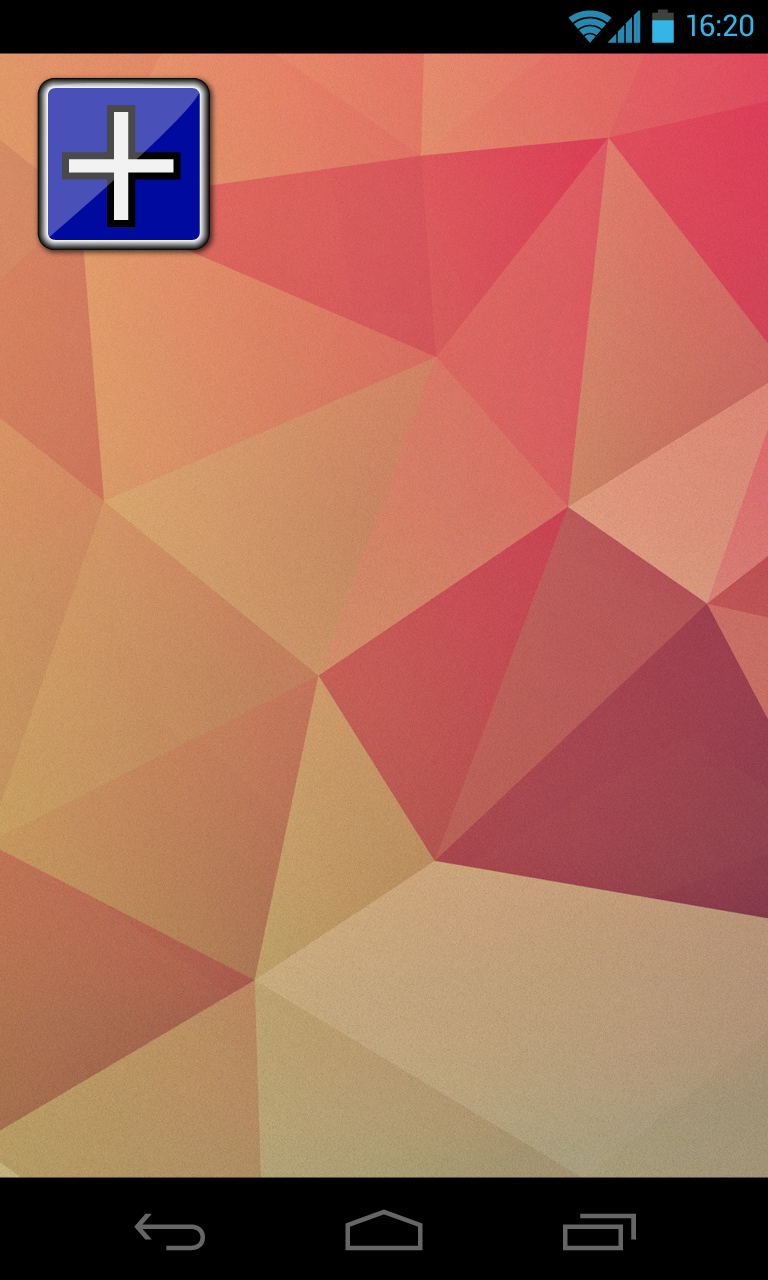
\includegraphics[scale=0.18]{Screens/00-Launch.png}

\includegraphics[scale=0.18]{Screens/00-Lock.png}
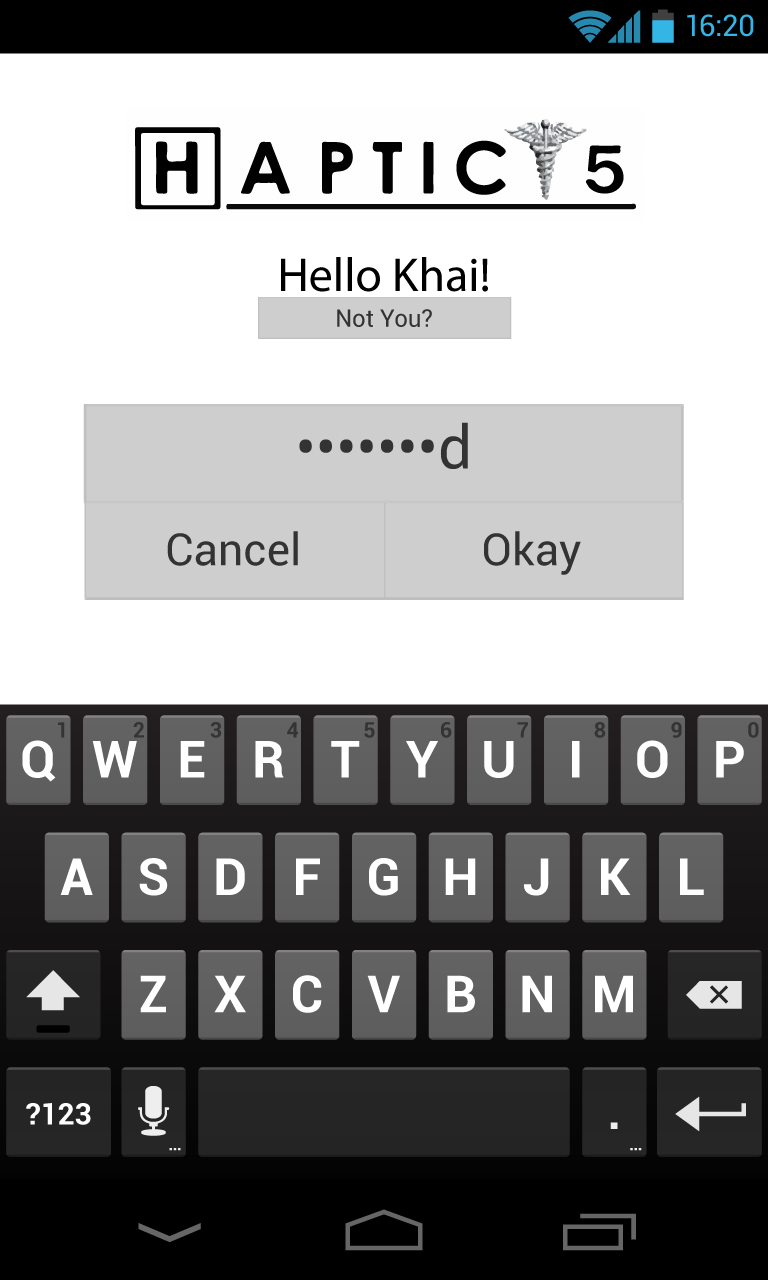
\includegraphics[scale=0.18]{Screens/00-Lock--Password-Entry.png}
\\\\
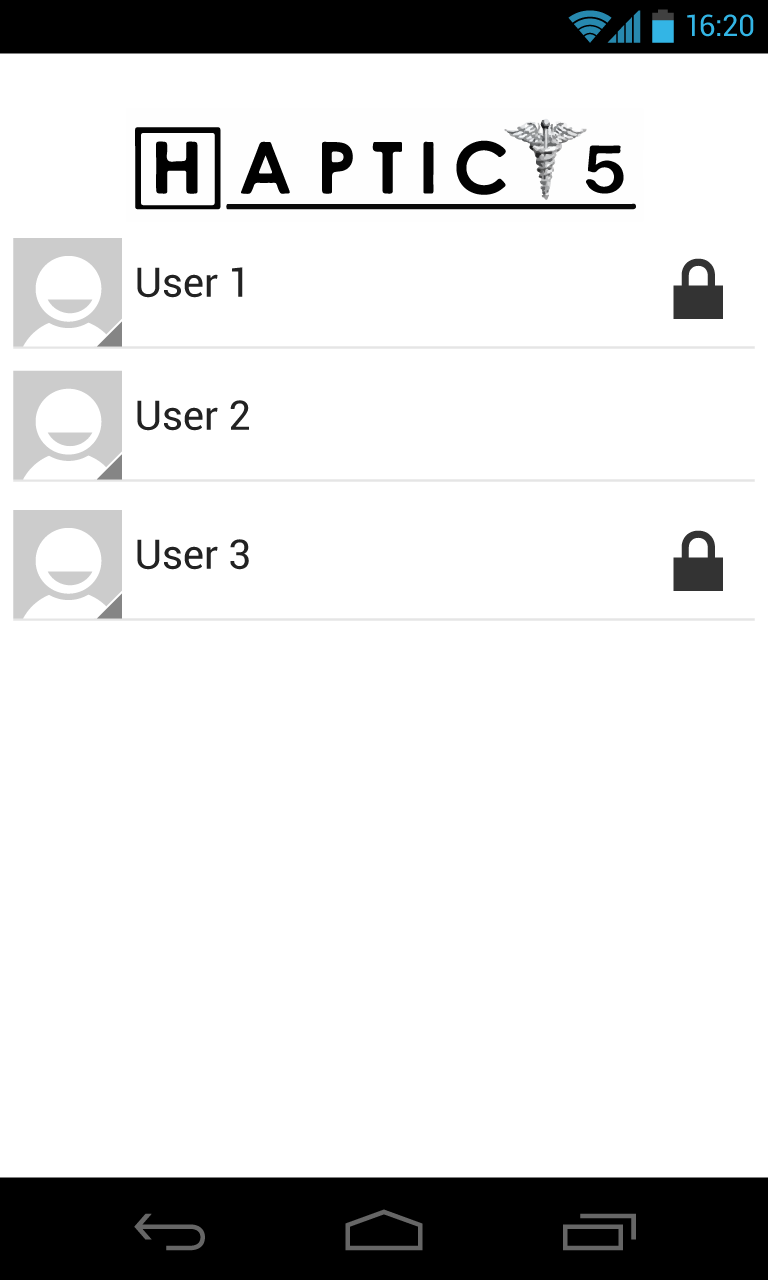
\includegraphics[scale=0.18]{Screens/01-Home---Change-User.png}
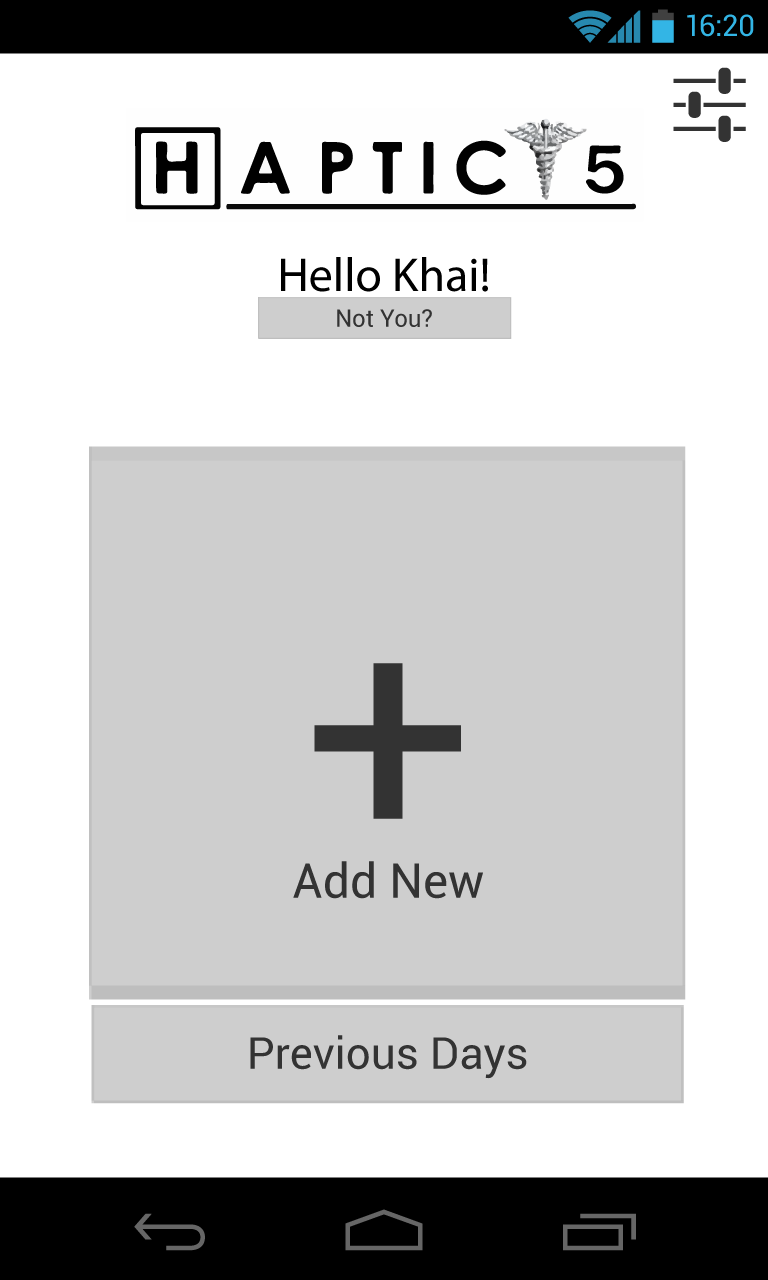
\includegraphics[scale=0.18]{Screens/01-Home---No-Selection.png}
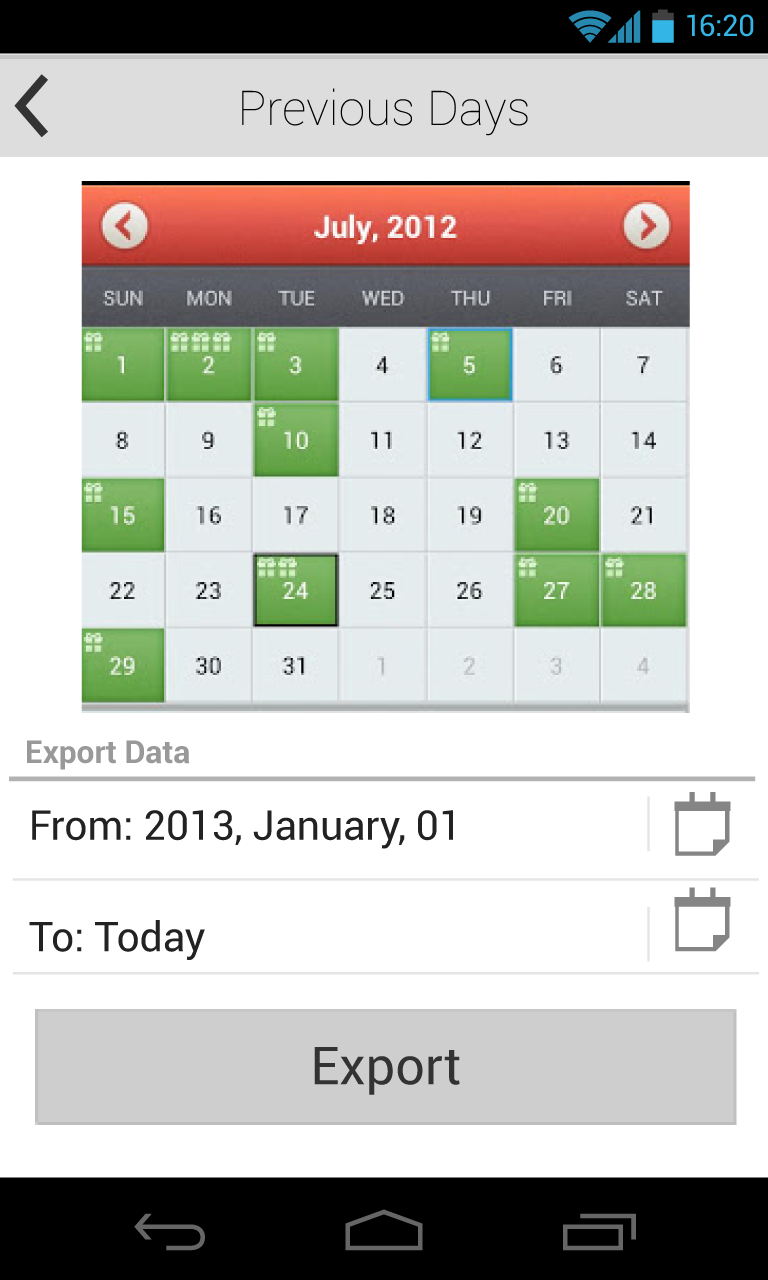
\includegraphics[scale=0.18]{Screens/02-Previous--No-Selection.png}
\\\\
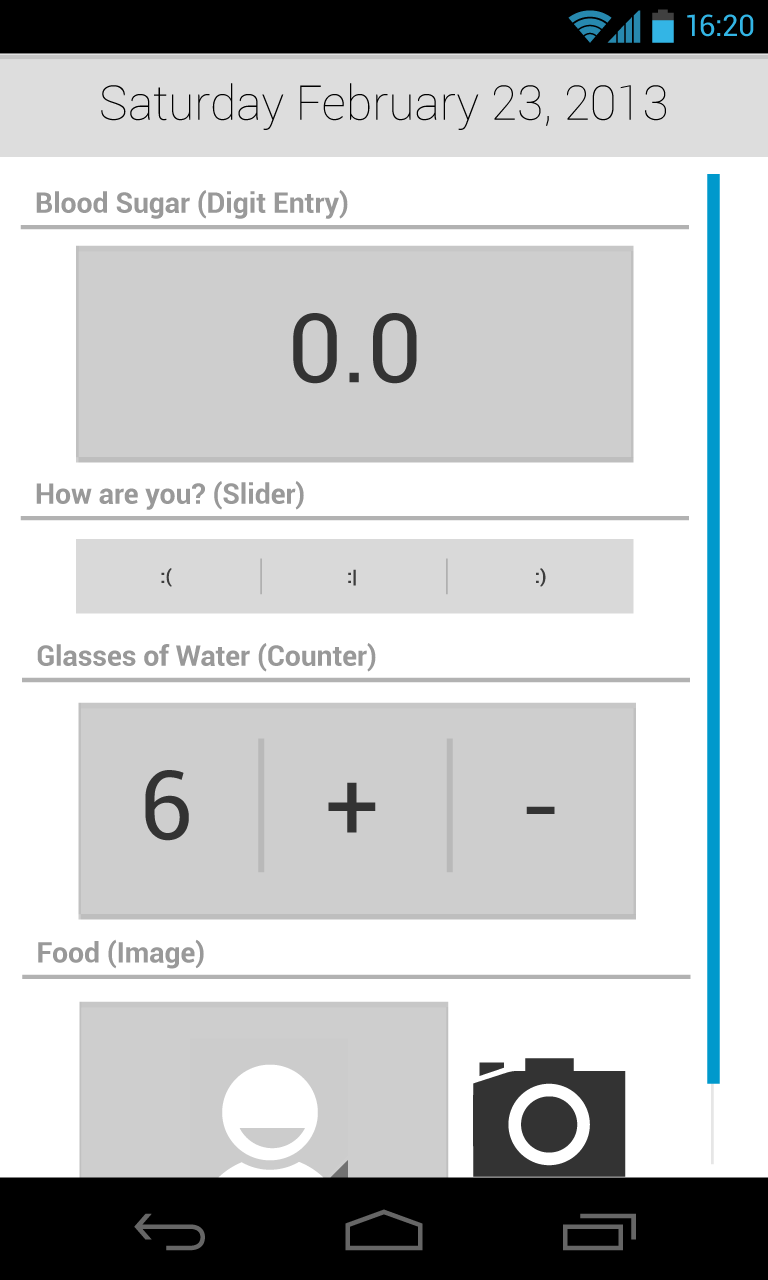
\includegraphics[scale=0.18]{Screens/03-Add--No-Selection.png}
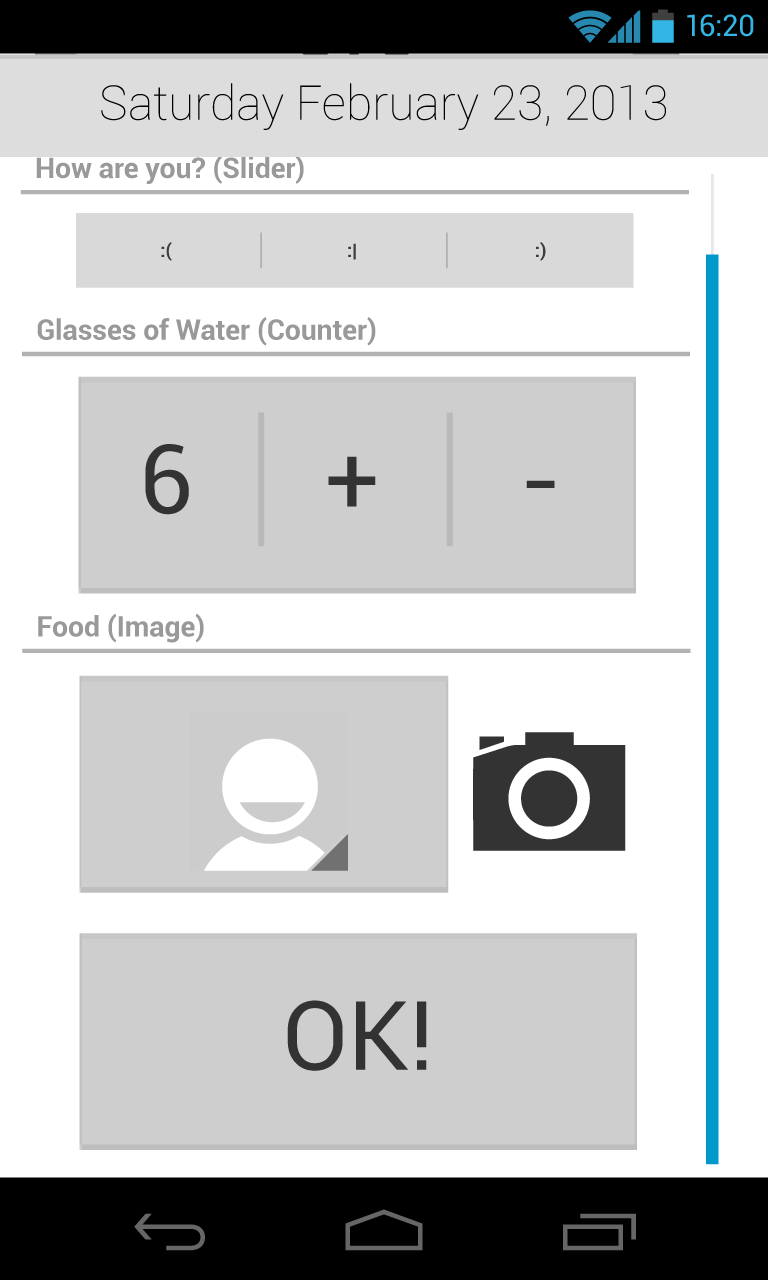
\includegraphics[scale=0.18]{Screens/03-Add--Scrolled.png}
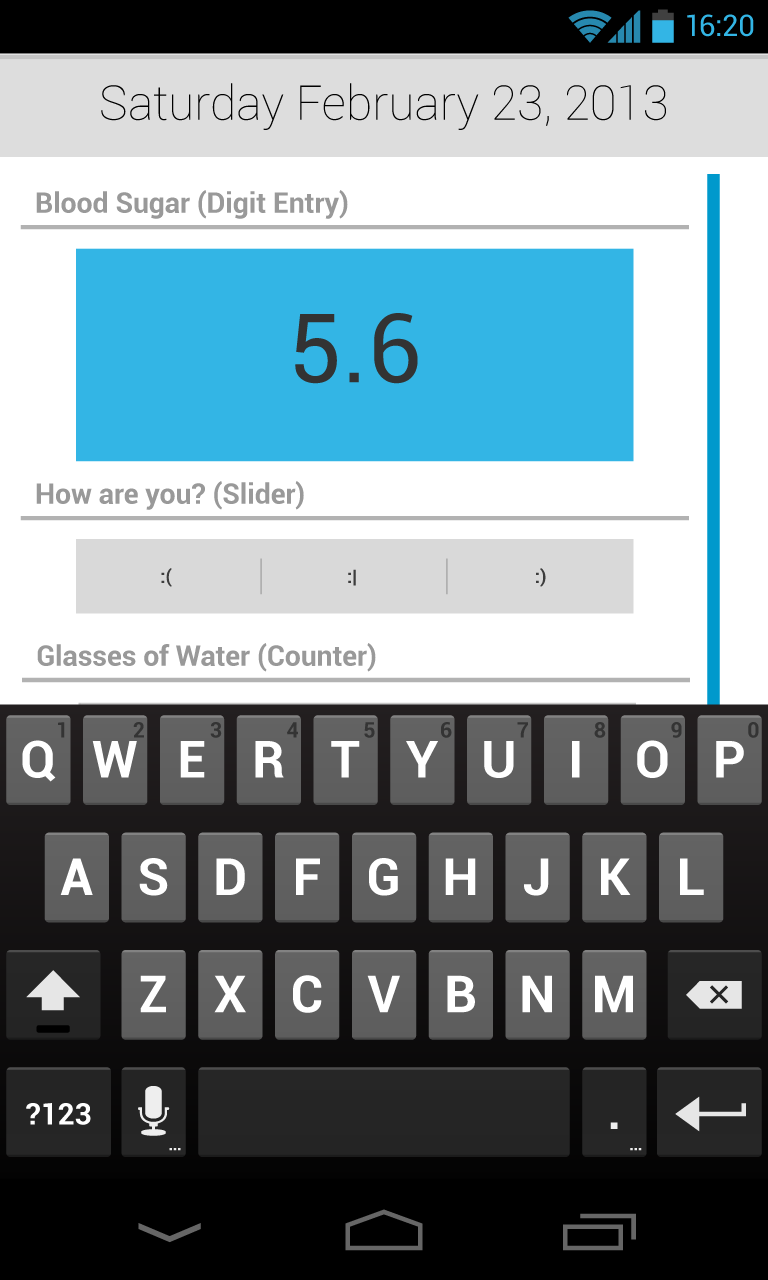
\includegraphics[scale=0.18]{Screens/03-Add--Add-Entry.png}
\\\\
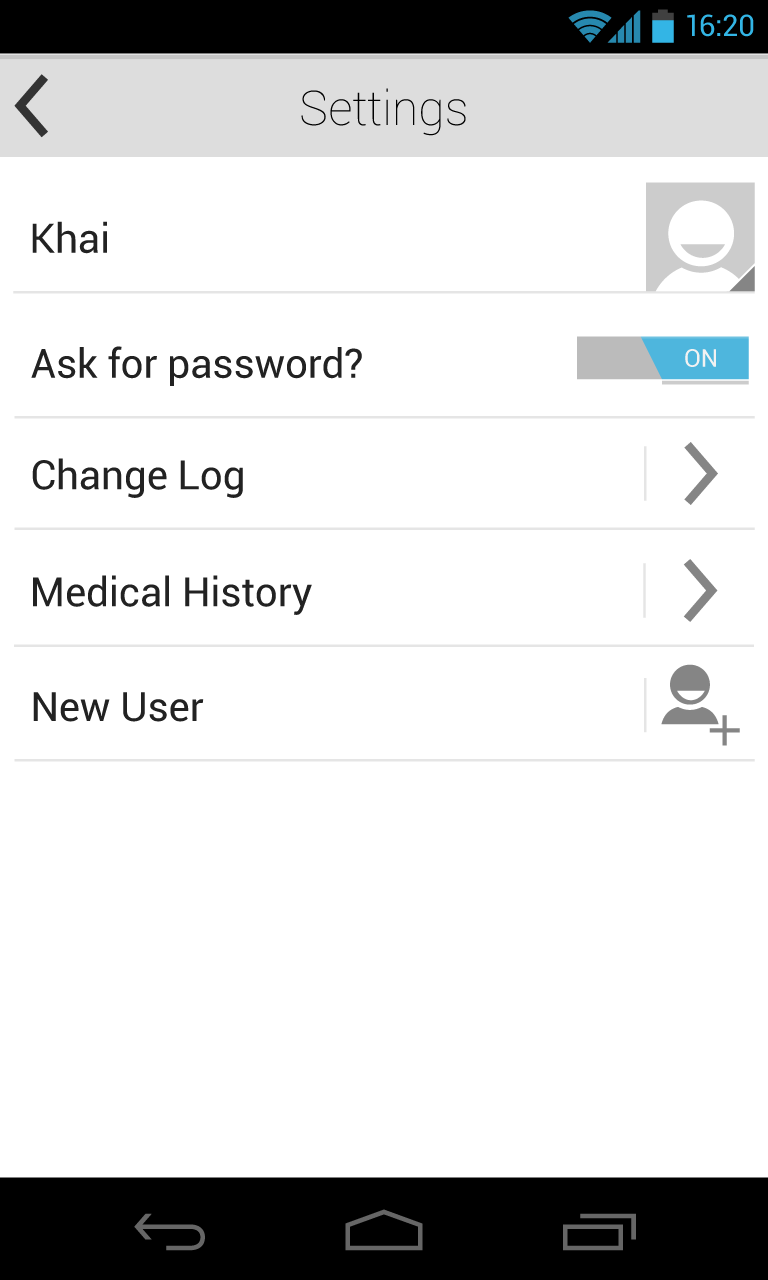
\includegraphics[scale=0.18]{Screens/04-Settings--Null.png}
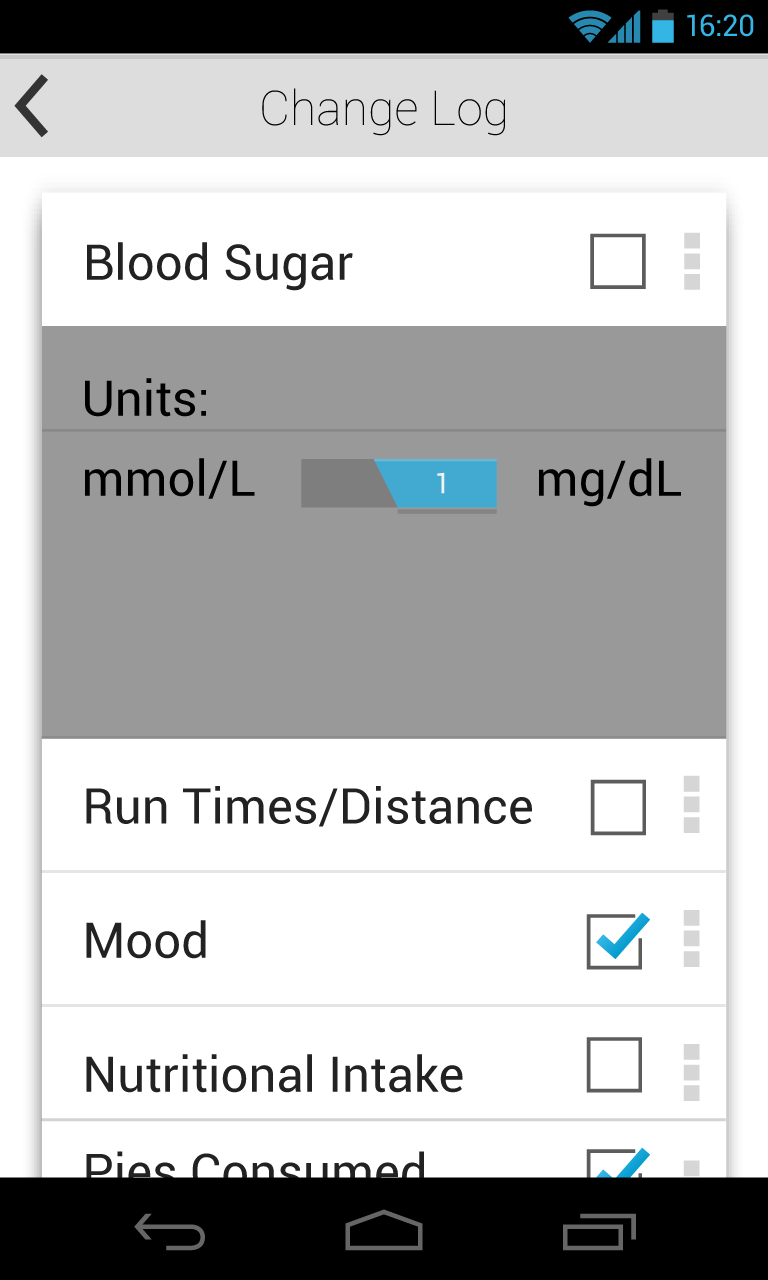
\includegraphics[scale=0.18]{Screens/05-Change-Log--Indi-Settings.png}
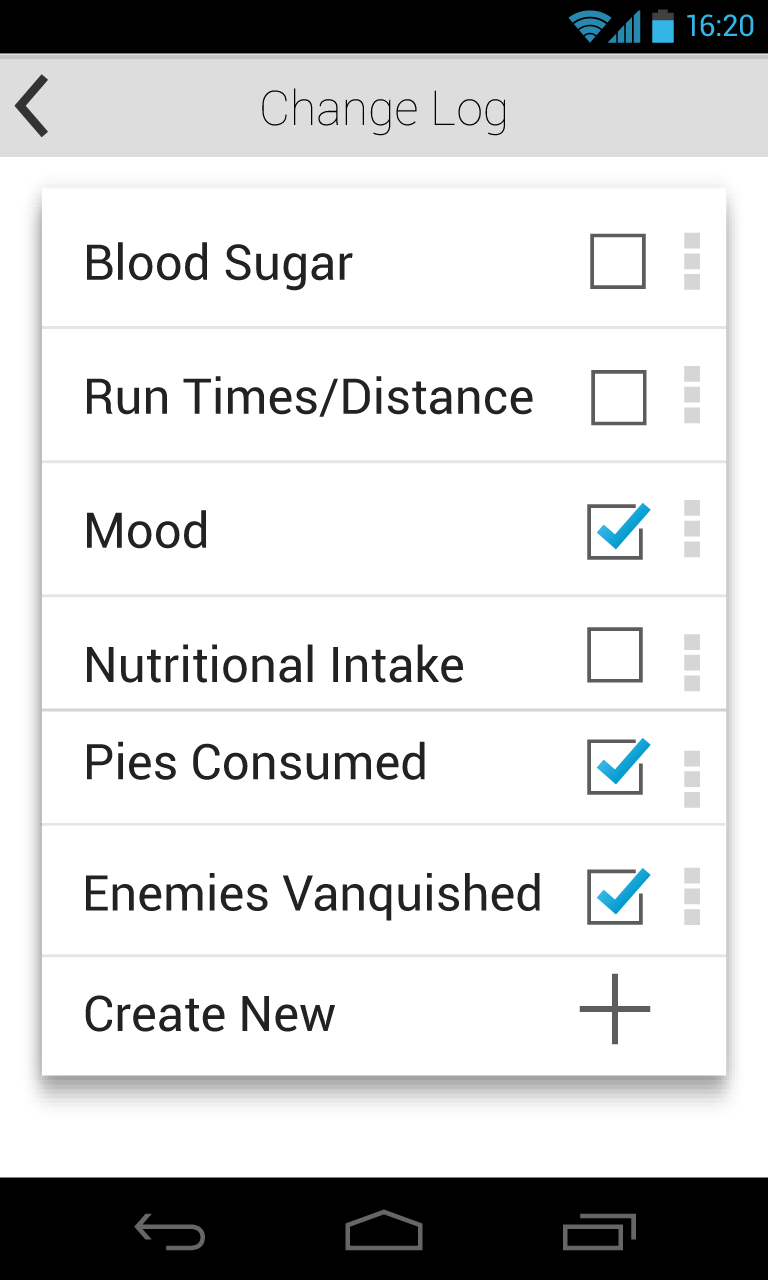
\includegraphics[scale=0.18]{Screens/05-Change-Log--Null.png}
\begin{enumerate}
\item{Phone Home Screen}
\item{Default User Screen (Password Protected)}
\item{Password Entry Screen}
\item{User Select Screen}
\item{User Home Screen}
\item{Previous Day Selection}
\item{Main Log Entry Screen}
\item{Main Log Entry Screen Scrolled Down}
\item{Selected Item Data Input}
\item{Settings Menu}
\item{Individual Category Customization}
\item{Category Menu}
\end{enumerate}
\section*{Sources}
http://www.cehd.umn.edu/nceo/OnlinePubs/Tech44/
\\http://www.nngroup.com/articles/thinking-aloud-the-1-usability-tool/




\end{document}
